

%%% This LaTeX source document can be used as the basis for your technical
%%% report. Intentionally stripped and simplified
%%% and commands should be adjusted for your particular paper - title, 
%%% author, citations, equations, etc.
% % Citations/references are in report.bib 

\documentclass[conference,backref=page]{acmsiggraph}

\TOGonlineid{45678}
\TOGvolume{0}
\TOGnumber{0}
\TOGarticleDOI{1111111.2222222}
\TOGprojectURL{}
\TOGvideoURL{}
\TOGdataURL{}
\TOGcodeURL{}

% Include this so that citations show up in blue and the page information is included in the reference section
\hypersetup{
    colorlinks = true, 
    linkcolor = blue,
    anchorcolor = red,
    citecolor = blue, 
    filecolor = red, 
}


\title{Milestone 2 Report}

\author{Neil Notman \thanks{e-mail:40124066@live.napier.ac.uk} \\
Edinburgh Napier University\\
Advanced Games Engineering(SET10110) \\
\url{http://nn1098.github.io/adved-games/github-pages/}}
\pdfauthor{Neil Notman}

\keywords{Game, Engine, racing, space}

\begin{document}

\teaser{
   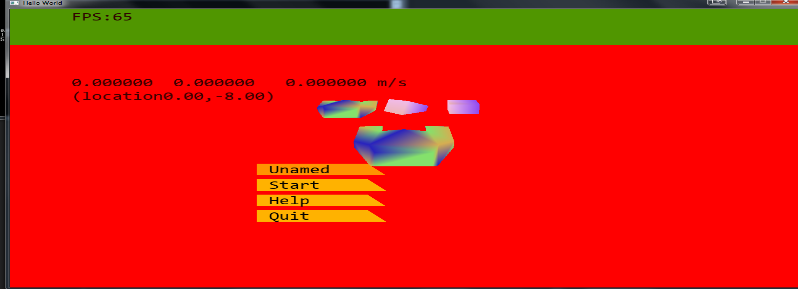
\includegraphics[height=1.5in]{images/mainmenu}
   \caption{This is the main menu screen of the game}
   \label{fig:mainmenu}
 }

\maketitle


\keywordlist

%% Use this only if you're preparing a technical paper to be published in the 
%% ACM 'Transactions on Graphics' journal.

% \TOGlinkslist

% \copyrightspace


\section{Introduction}
The aim of this report and following implementation is to create a game with that conforms to industry standards and contains an agreed list of key functions the report will be used to detail current features and list future work for the next milestone.

This project was initially based as a group however this has now been reduced to a solo implementation which has strained the developement process however the focus for the remainder of the project will be on key features for playability of the game.     

The game itself is currently unnamed but the original idea was for the game to be a 3d space based racer with area's for both racing and free flight with multi-player functionality  

\section{Current features}
The game currently features a full menu system and debug overlay as shown in \ref{fig:mainmenu} in terms of graphical content there is model loading and rendering functionality with a variety of basic shaders. 

There are multiple input methods including command parsing using the command line there is also gamepad input and keyboard handling which allows for movement of the player with velocity based integration. 


The red plane shown in \ref{fig:mainmenu} is redrawn based on the current 
\section{features for milestone 3}


\section{Conclusion}



% \section*{Acknowledgements}
\bibliographystyle{acmsiggraph}
\bibliography{report}

\end{document}

